\documentclass[11pt,a4paper]{article}
\usepackage[margin=2.5cm]{geometry}
\usepackage{graphicx}

\title{Labwork 5: Gaussian Blur}
\author{Duong Tan Binh \\ Student ID: 2540007}
\date{}

\begin{document}
\maketitle

\section{CPU}
I use the 512 by 600 grayscale image from Lab 4.
For each pixel, I multiply its 7 by 7 neighbourhood by the filter
from the slide and add the results. The filter values sum to 1003,
so I divide the total by 1003 and keep the integer part.
At the image edges, I repeat the nearest pixel.
The CPU version uses loops over the pixels and filter entries.

\section{GPU global memory}
I keep the 2D thread indices from Lab 4. Each thread calculates
one output pixel with the same loops as the CPU.
The image and filter are read from global memory.
I test blocks of 8 by 8, 16 by 16 and 32 by 32 threads.

\section{GPU shared memory}
In each block, 49 threads copy the 49 filter values into shared memory.
All threads in the block call \texttt{cuda.syncthreads()} before using them.
The blur calculation stays the same. Only the filter is in shared memory;
the image stays in global memory.

\section{Results}
I use \texttt{time.time()} and measure each configuration once.
Each GPU kernel runs once before timing to exclude compilation.
GPU time includes copying the image in and the result out.
The initial allocation and filter upload are outside the timer.
Speedup is CPU time divided by GPU time.

\begin{verbatim}
CPU: 6842.816 ms

Global 8x8: 0.500 ms, speedup 13693.15
Global 16x16: 0.348 ms, speedup 19685.08
Global 32x32: 0.334 ms, speedup 20515.26

Shared 8x8: 0.461 ms, speedup 14840.15
Shared 16x16: 0.364 ms, speedup 18783.28
Shared 32x32: 0.309 ms, speedup 22128.64
\end{verbatim}
The CPU and both GPU versions give the same output values.

\newpage
\section{Comparison}
\begin{center}
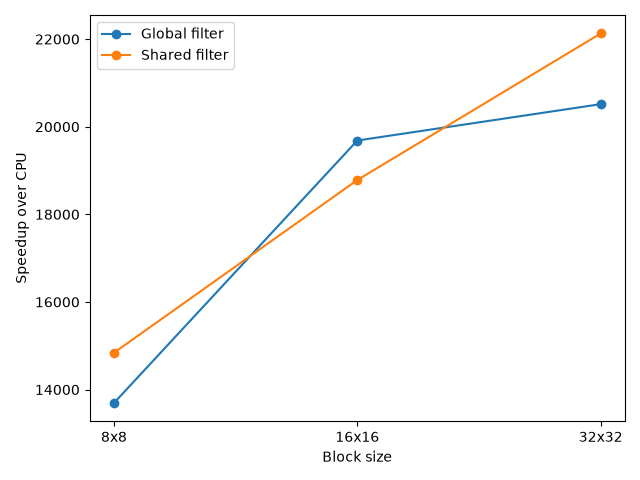
\includegraphics[width=0.75\textwidth]{block_size_speedup.png}
\end{center}
The 32 by 32 block is fastest for both GPU versions in this run.
Shared memory is faster at 8 by 8 and 32 by 32, but slightly slower
at 16 by 16. Copying the filter and waiting for the block also take time.
These single measurements do not show that shared memory is always faster.
The large speedups are relative to Python loops on the CPU, not an
optimized CPU blur function.

\begin{center}
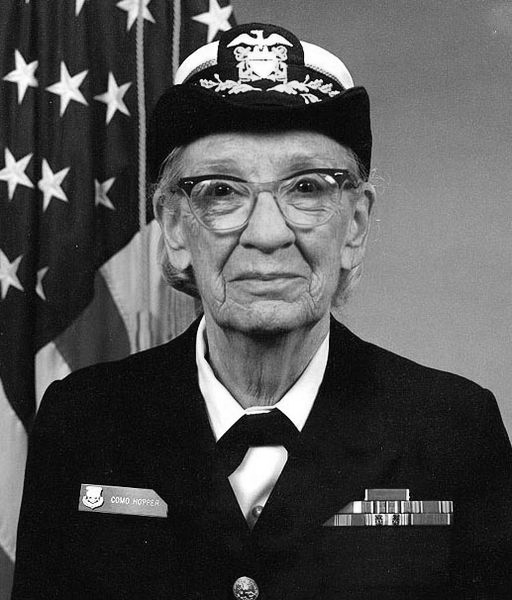
\includegraphics[width=0.22\textwidth]{input.png}
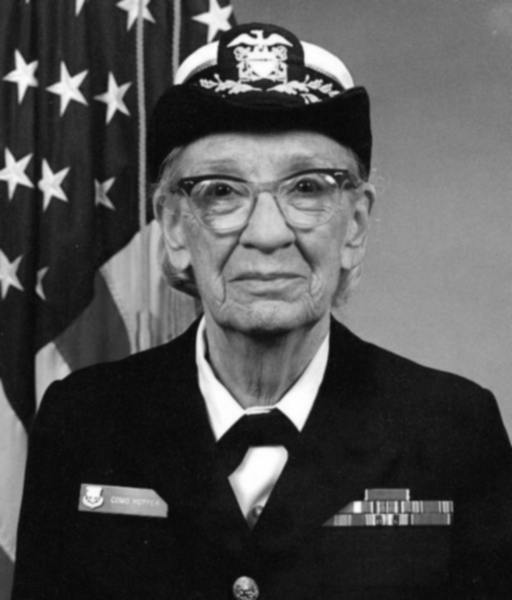
\includegraphics[width=0.22\textwidth]{blur_cpu.png}
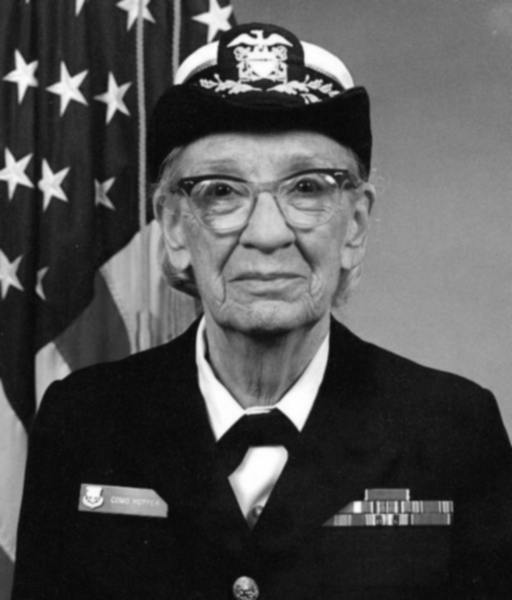
\includegraphics[width=0.22\textwidth]{blur_global.png}
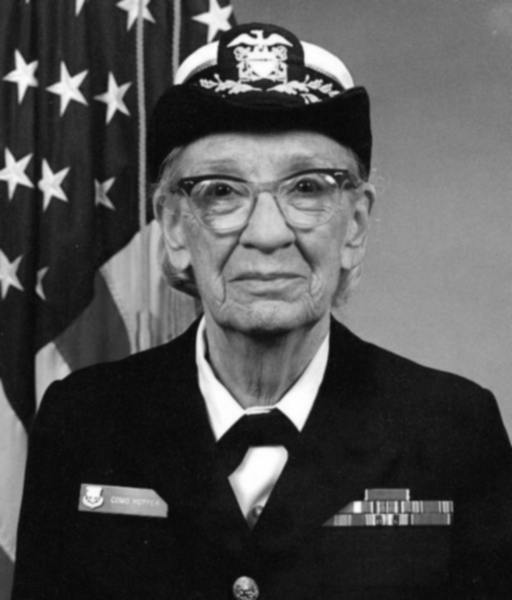
\includegraphics[width=0.22\textwidth]{blur_shared.png}
\end{center}
From left to right: input, CPU blur, GPU global blur, GPU shared blur.

\end{document}
